% Options for packages loaded elsewhere
\PassOptionsToPackage{unicode}{hyperref}
\PassOptionsToPackage{hyphens}{url}
%
\documentclass[
  ignorenonframetext,
  aspectratio=169,
]{beamer}
\usepackage{pgfpages}
\setbeamertemplate{caption}[numbered]
\setbeamertemplate{caption label separator}{: }
\setbeamercolor{caption name}{fg=normal text.fg}
\beamertemplatenavigationsymbolsempty
% Prevent slide breaks in the middle of a paragraph
\widowpenalties 1 10000
\raggedbottom
\setbeamertemplate{part page}{
  \centering
  \begin{beamercolorbox}[sep=16pt,center]{part title}
    \usebeamerfont{part title}\insertpart\par
  \end{beamercolorbox}
}
\setbeamertemplate{section page}{
  \centering
  \begin{beamercolorbox}[sep=12pt,center]{part title}
    \usebeamerfont{section title}\insertsection\par
  \end{beamercolorbox}
}
\setbeamertemplate{subsection page}{
  \centering
  \begin{beamercolorbox}[sep=8pt,center]{part title}
    \usebeamerfont{subsection title}\insertsubsection\par
  \end{beamercolorbox}
}
\AtBeginPart{
  \frame{\partpage}
}
\AtBeginSection{
  \ifbibliography
  \else
    \frame{\sectionpage}
  \fi
}
\AtBeginSubsection{
  \frame{\subsectionpage}
}

\usepackage{amsmath,amssymb}
\usepackage{iftex}
\ifPDFTeX
  \usepackage[T1]{fontenc}
  \usepackage[utf8]{inputenc}
  \usepackage{textcomp} % provide euro and other symbols
\else % if luatex or xetex
  \usepackage{unicode-math}
  \defaultfontfeatures{Scale=MatchLowercase}
  \defaultfontfeatures[\rmfamily]{Ligatures=TeX,Scale=1}
\fi
\usepackage{lmodern}
\usetheme[]{default}
\ifPDFTeX\else  
    % xetex/luatex font selection
\fi
% Use upquote if available, for straight quotes in verbatim environments
\IfFileExists{upquote.sty}{\usepackage{upquote}}{}
\IfFileExists{microtype.sty}{% use microtype if available
  \usepackage[]{microtype}
  \UseMicrotypeSet[protrusion]{basicmath} % disable protrusion for tt fonts
}{}
\makeatletter
\@ifundefined{KOMAClassName}{% if non-KOMA class
  \IfFileExists{parskip.sty}{%
    \usepackage{parskip}
  }{% else
    \setlength{\parindent}{0pt}
    \setlength{\parskip}{6pt plus 2pt minus 1pt}}
}{% if KOMA class
  \KOMAoptions{parskip=half}}
\makeatother
\usepackage{xcolor}
\newif\ifbibliography
\setlength{\emergencystretch}{3em} % prevent overfull lines
\setcounter{secnumdepth}{-\maxdimen} % remove section numbering


\providecommand{\tightlist}{%
  \setlength{\itemsep}{0pt}\setlength{\parskip}{0pt}}\usepackage{longtable,booktabs,array}
\usepackage{calc} % for calculating minipage widths
\usepackage{caption}
% Make caption package work with longtable
\makeatletter
\def\fnum@table{\tablename~\thetable}
\makeatother
\usepackage{graphicx}
\makeatletter
\def\maxwidth{\ifdim\Gin@nat@width>\linewidth\linewidth\else\Gin@nat@width\fi}
\def\maxheight{\ifdim\Gin@nat@height>\textheight\textheight\else\Gin@nat@height\fi}
\makeatother
% Scale images if necessary, so that they will not overflow the page
% margins by default, and it is still possible to overwrite the defaults
% using explicit options in \includegraphics[width, height, ...]{}
\setkeys{Gin}{width=\maxwidth,height=\maxheight,keepaspectratio}
% Set default figure placement to htbp
\makeatletter
\def\fps@figure{htbp}
\makeatother

\usepackage{tikz}
\usetikzlibrary{arrows.meta,positioning}
\usepackage{booktabs}

% ======================================================================
%  EDIT BLOCK 2 of 2: the classification banner.
% ======================================================================
\newcommand{\classification}{UNCLASSIFIED}
\definecolor{classbg}{HTML}{006400}
% ======================================================================

\definecolor{vpurple}{HTML}{440154}
\definecolor{vteal}{HTML}{21918C}
\definecolor{vgreen}{HTML}{5EC962}

\setbeamercolor{classbanner}{bg=classbg,fg=white}
\setbeamercolor{frametitle}{fg=vpurple,bg=white}
\setbeamercolor{title}{fg=vpurple}
\setbeamercolor{structure}{fg=vteal}
\setbeamertemplate{navigation symbols}{}

\setbeamertemplate{headline}{%
  \begin{beamercolorbox}[wd=\paperwidth,ht=2.0ex,dp=0.7ex,center]{classbanner}%
    \bfseries\small\classification%
  \end{beamercolorbox}%
}
\setbeamertemplate{footline}{%
  \begin{beamercolorbox}[wd=\paperwidth,ht=2.0ex,dp=0.7ex]{classbanner}%
    \hspace*{2ex}\bfseries\small\insertframenumber\hfill\classification\hfill\hspace*{2ex}%
  \end{beamercolorbox}%
}

% The bottom line for each slide. One sentence: what is happening, why.
\newcommand{\bottomline}[1]{\par\noindent{\small\color{vpurple}\textbf{#1}}\par\vspace{0.6em}}
\newcommand{\kicker}[1]{\par\noindent{\footnotesize\color{vteal}\textbf{\MakeUppercase{#1}}}\par\vspace{0.3em}}

% Uncomment to project speaker notes on a second screen:
% \setbeameroption{show notes on second screen=right}
\makeatletter
\@ifpackageloaded{caption}{}{\usepackage{caption}}
\AtBeginDocument{%
\ifdefined\contentsname
  \renewcommand*\contentsname{Table of contents}
\else
  \newcommand\contentsname{Table of contents}
\fi
\ifdefined\listfigurename
  \renewcommand*\listfigurename{List of Figures}
\else
  \newcommand\listfigurename{List of Figures}
\fi
\ifdefined\listtablename
  \renewcommand*\listtablename{List of Tables}
\else
  \newcommand\listtablename{List of Tables}
\fi
\ifdefined\figurename
  \renewcommand*\figurename{Figure}
\else
  \newcommand\figurename{Figure}
\fi
\ifdefined\tablename
  \renewcommand*\tablename{Table}
\else
  \newcommand\tablename{Table}
\fi
}
\@ifpackageloaded{float}{}{\usepackage{float}}
\floatstyle{ruled}
\@ifundefined{c@chapter}{\newfloat{codelisting}{h}{lop}}{\newfloat{codelisting}{h}{lop}[chapter]}
\floatname{codelisting}{Listing}
\newcommand*\listoflistings{\listof{codelisting}{List of Listings}}
\makeatother
\makeatletter
\makeatother
\makeatletter
\@ifpackageloaded{caption}{}{\usepackage{caption}}
\@ifpackageloaded{subcaption}{}{\usepackage{subcaption}}
\makeatother

\ifLuaTeX
  \usepackage{selnolig}  % disable illegal ligatures
\fi
\usepackage{bookmark}

\IfFileExists{xurl.sty}{\usepackage{xurl}}{} % add URL line breaks if available
\urlstyle{same} % disable monospaced font for URLs
\hypersetup{
  pdftitle={Measuring What We Never Asked},
  pdfauthor={Kevin Linares},
  hidelinks,
  pdfcreator={LaTeX via pandoc}}


\title{Measuring What We Never Asked}
\subtitle{Grouping survey items into population inferences, with the
sample design carried through}
\author{Kevin Linares}
\date{3 August 2026}
\institute{Public Opinion Research}

\begin{document}
\frame{\titlepage}


\begin{frame}[shrink]{This project started with a battery and no
principled way to summarize it}
\phantomsection\label{this-project-started-with-a-battery-and-no-principled-way-to-summarize-it}
\bottomline{We field 11 items to measure something no respondent answers directly, and how we combine them has always been settled by convention rather than by evidence.}

\begin{columns}[T]
\begin{column}{0.52\textwidth}
\kicker{the two defaults}
\small
\begin{itemize}\itemsep4pt
  \item \textbf{Average them into an index.} Readable, but it assumes every respondent differs from every other only in \emph{how much}.
  \item \textbf{Report all 11 separately.} Faithful, but no policymaker product can carry 11 lines, so someone collapses them anyway, off the record.
\end{itemize}
\end{column}
\begin{column}{0.44\textwidth}
\kicker{the question nobody had tested}
\small
Is the index a summary of the battery, or an artifact of the decision to build one?

\vspace{0.5em}

That is an empirical question. This project answers it, and carries the sample design through the answer.
\end{column}
\end{columns}

\note{Ninety seconds. Name the concrete request that started this: someone asked for one number off this battery for a country product. Both available answers were defaults nobody had ever checked. Do not defend the method yet.}
\end{frame}

\begin{frame}[shrink]{Nobody in our data was ever asked the question we
report on}
\phantomsection\label{nobody-in-our-data-was-ever-asked-the-question-we-report-on}
\bottomline{Every statement we publish about economic vulnerability is an inference from proxies, and its quality depends entirely on how those proxies are combined.}

\vspace{0.3em}

\begin{center}
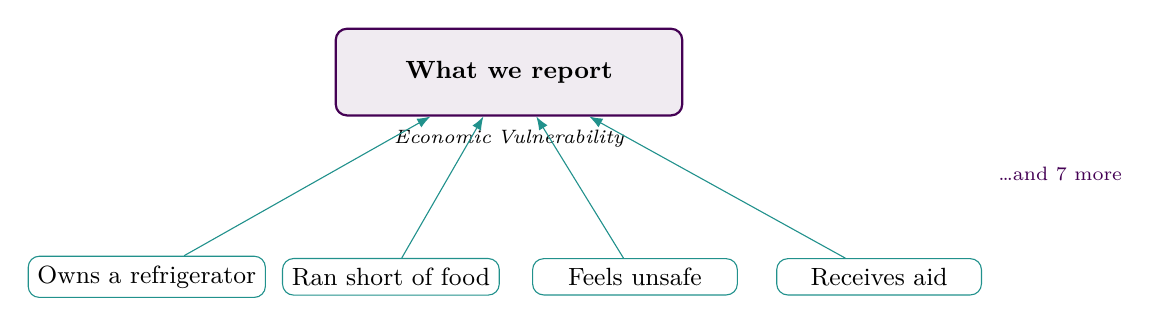
\begin{tikzpicture}[font=\small]
  \node[draw=vpurple,thick,rounded corners,fill=vpurple!8,minimum width=4.4cm,minimum height=1.1cm] (concept) at (0,0) {\textbf{What we report}};
  \node[below=0.05cm of concept,text width=4.4cm,align=center,font=\scriptsize\itshape] {Economic Vulnerability};
  \node[draw=vteal,rounded corners,minimum width=2.6cm] (i1) at (-4.6,-2.6) {Owns a refrigerator};
  \node[draw=vteal,rounded corners,minimum width=2.6cm] (i2) at (-1.5,-2.6) {Ran short of food};
  \node[draw=vteal,rounded corners,minimum width=2.6cm] (i3) at (1.6,-2.6) {Feels unsafe};
  \node[draw=vteal,rounded corners,minimum width=2.6cm] (i4) at (4.7,-2.6) {Receives aid};
  \draw[-{Latex},vteal] (i1) -- (concept);
  \draw[-{Latex},vteal] (i2) -- (concept);
  \draw[-{Latex},vteal] (i3) -- (concept);
  \draw[-{Latex},vteal] (i4) -- (concept);
  \node[font=\scriptsize,text=vpurple] at (7.0,-1.3) {\ldots and 7 more};
\end{tikzpicture}
\end{center}

\vspace{0.2em}

\centering\small On what basis do we decide that these 11 answers add up
to that one thing?

\note{This is the hook. Say the concept out loud, then say no one was asked it. Ask the question on the last line and pause. Do not answer it yet. Swap the four item labels for the ones on the country account.}
\end{frame}

\begin{frame}[shrink]{A battery can differ in degree or in kind, and
only one summary is right}
\phantomsection\label{a-battery-can-differ-in-degree-or-in-kind-and-only-one-summary-is-right}
\bottomline{If people differ in how much, one scale describes them; if they differ in which answers they favor, that scale averages opposite people into a middle where nobody actually sits.}

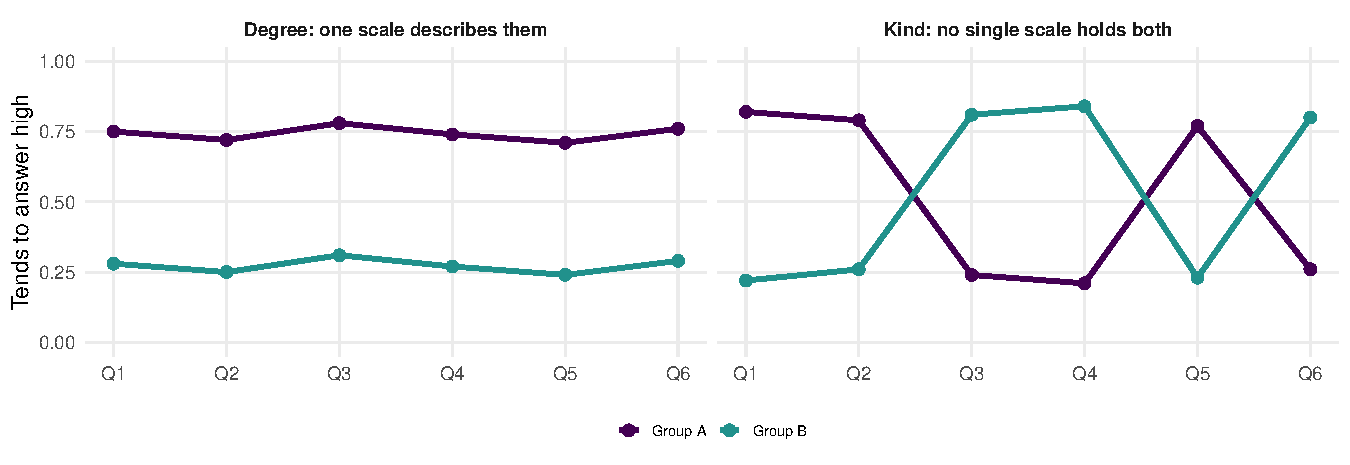
\includegraphics[width=1\textwidth,height=\textheight]{lca_briefing_files/figure-beamer/fork-figure-1.pdf}

\centering\small Which picture our battery matches is a question the
data can answer. Until now we have answered it by assumption.

\note{No real data on this slide on purpose. Left panel: an index is fine, the groups differ only in level. Right panel: the lines cross, an index puts both groups at the same middling number. Forty-five seconds.}
\end{frame}

\begin{frame}[shrink]{Roadmap}
\phantomsection\label{roadmap}
\bottomline{You have the question; here is the order in which the rest of this answers it.}

\vspace{0.5em}

\begin{columns}[T]
\begin{column}{0.52\textwidth}
\begin{enumerate}\itemsep5pt
  \item \textbf{What we found} on AmericasBarometer 2023, Ecuador
  \item \textbf{How the method decides} degree versus kind
  \item \textbf{Why the sample design} changes the answer
  \item \textbf{Where AI fits}, and where it must not
  \item \textbf{What I need from you}: how to capture this in production
\end{enumerate}
\end{column}
\begin{column}{0.44\textwidth}
\small
\textbf{The claim in one line}

\vspace{0.4em}

Grouping survey items into a population inference is a measurement decision and a design decision at once. Doing either alone gives a number we cannot defend.
\end{column}
\end{columns}

\note{Thirty seconds, no more. The roadmap is here rather than up front because slides 1 to 3 gave it something to organize.}
\end{frame}

\begin{frame}[shrink]{On AmericasBarometer 2023, Ecuador, the answer is
kind, not degree}
\phantomsection\label{on-americasbarometer-2023-ecuador-the-answer-is-kind-not-degree}
\bottomline{The battery does not line respondents up on one scale; it separates them into 4 recognizable groups, which means an index built from it has been averaging distinct publics together.}

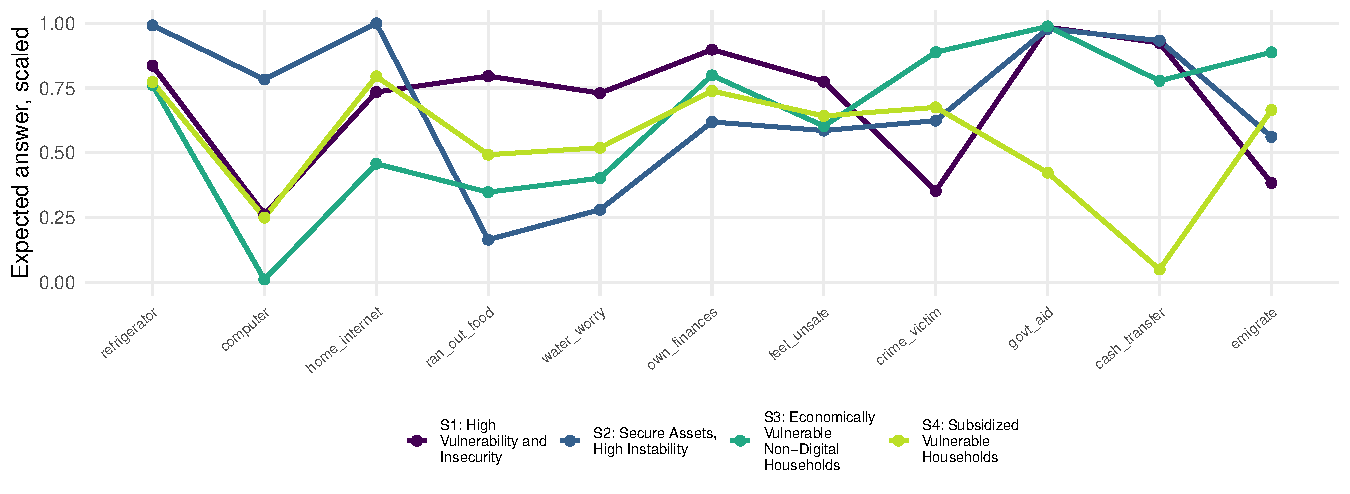
\includegraphics[width=1\textwidth,height=\textheight]{lca_briefing_files/figure-beamer/profiles-1.pdf}

\centering\small Lines that cross are the evidence: these groups reorder
the items rather than sitting above and below each other.

\note{The payoff. Walk two segments only, by name, and point at one crossing. Resist naming all of them. Sixty seconds.}
\end{frame}

\begin{frame}[shrink]{These are population shares, not clusters that
exist only in this file}
\phantomsection\label{these-are-population-shares-not-clusters-that-exist-only-in-this-file}
\bottomline{Each segment is estimated as a share of the adult population with its own margin of error, so these are numbers a product can carry.}

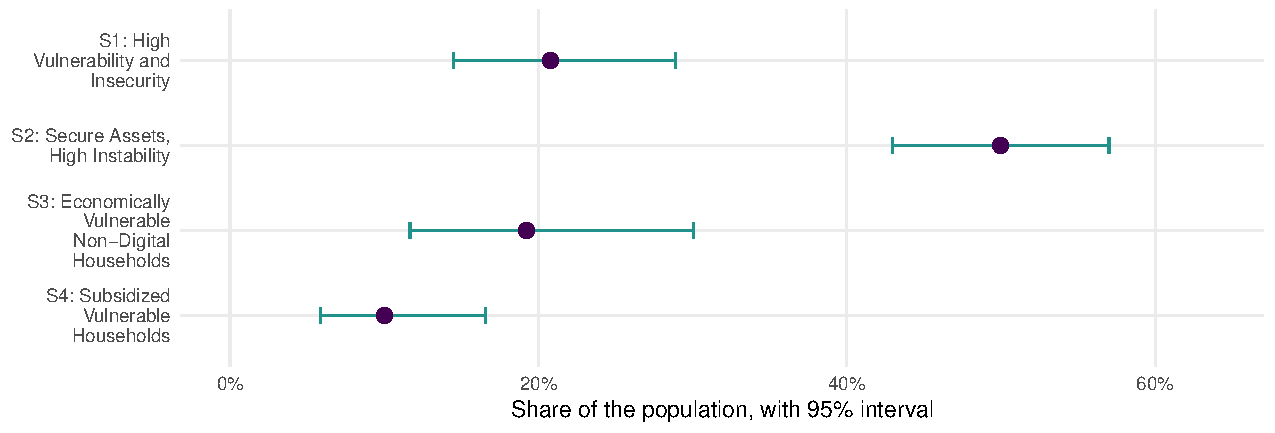
\includegraphics[width=0.95\textwidth,height=\textheight]{lca_briefing_files/figure-beamer/prevalences-1.pdf}

\small The largest segment is 50\% of adults (43 to 57\%); the smallest
is 10\%. Intervals come from the sample design, not from a formula that
assumes independent respondents.

\note{The word to land is population. A cluster analysis gives you groups in this file; this gives you shares of the country with uncertainty attached. Forty-five seconds.}
\end{frame}

\begin{frame}[shrink]{The segments cut across age group in ways the
toplines hide}
\phantomsection\label{the-segments-cut-across-age-group-in-ways-the-toplines-hide}
\bottomline{Groups that look similar on a topline concentrate in different segments, which is why subgroup trends built on an index have looked flat.}

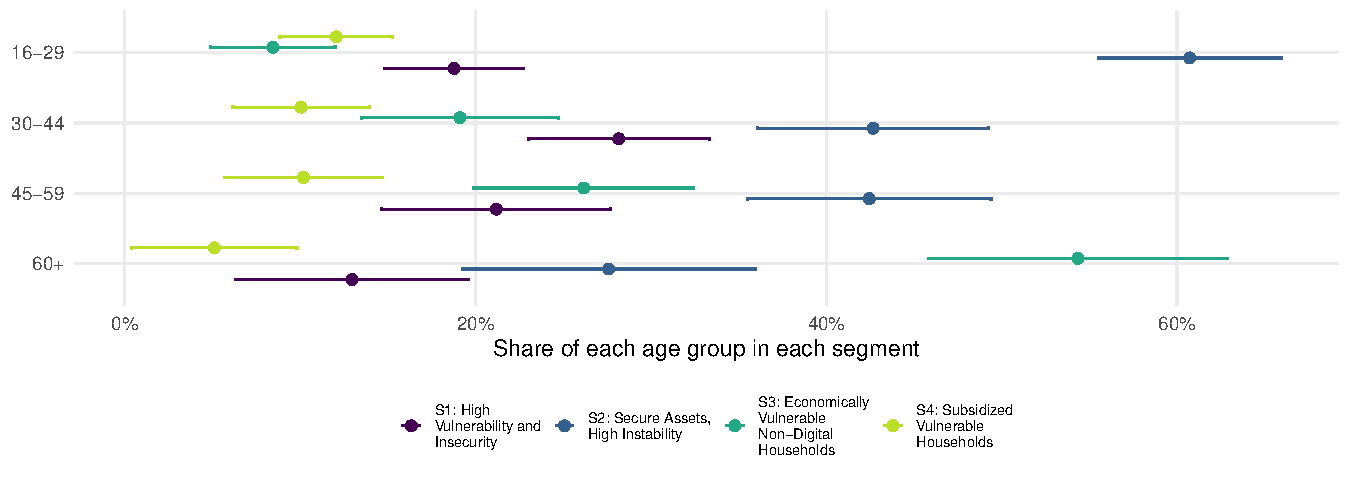
\includegraphics[width=1\textwidth,height=\textheight]{lca_briefing_files/figure-beamer/demo-composition-1.pdf}

\note{Their standard cross-tab, showing something their standard cross-tab cannot. Name one contrast that would change a country product. Sixty seconds.}
\end{frame}

\begin{frame}[shrink]{What we would have reported, and what the data
support}
\phantomsection\label{what-we-would-have-reported-and-what-the-data-support}
\bottomline{Reading across the three versions shows first what ignoring the sample design costs, then what forcing each respondent into one box costs, and the second gap is the larger one.}

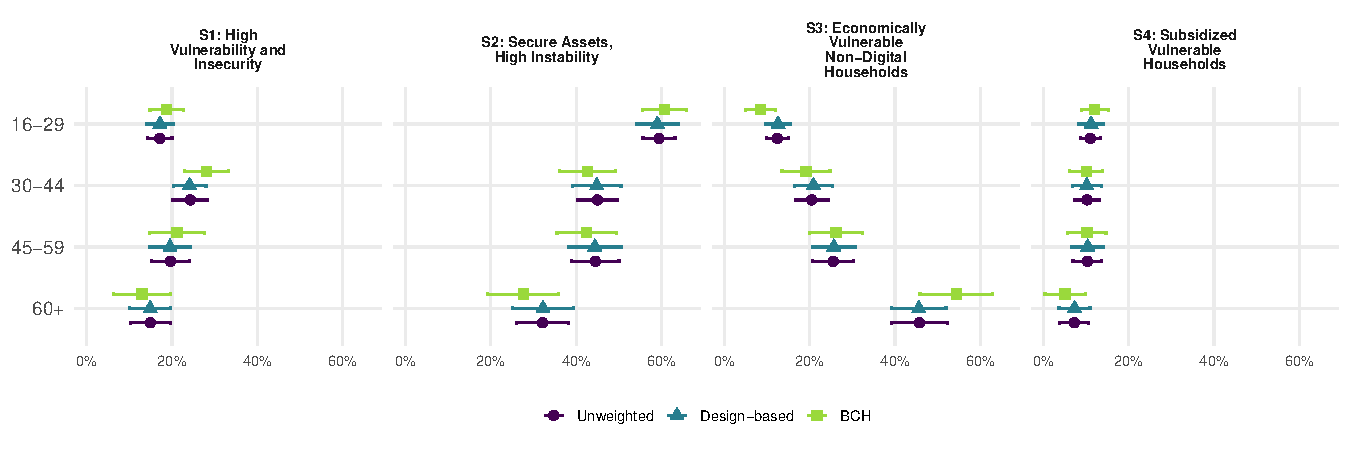
\includegraphics[width=1\textwidth,height=\textheight]{lca_briefing_files/figure-beamer/three-estimators-1.pdf}

\small\textbf{Unweighted} is the plain cross-tab. \textbf{Design-based}
adds the weights and the clustering. \textbf{Corrected} additionally
undoes the shrinkage that assigning each respondent to one segment
introduces.

\note{Do not explain BCH here. The point is that the three rows are different and only the third is defensible. If asked how the correction works, go to backup. Sixty seconds.}
\end{frame}

\begin{frame}[shrink]{The method groups respondents by pattern, not by
score}
\phantomsection\label{the-method-groups-respondents-by-pattern-not-by-score}
\bottomline{A latent class model asks which answers travel together, so it can find people who are secure on some items and exposed on others, which a scale cannot represent.}

\begin{columns}[T]
\begin{column}{0.50\textwidth}
\kicker{what the model estimates}
\small
\begin{itemize}\itemsep3pt
  \item How many kinds of respondent there are
  \item For each kind, the probability of every answer to every item
  \item For each respondent, which kind they most resemble, and how sure we are
\end{itemize}
\end{column}
\begin{column}{0.46\textwidth}
\kicker{why it suits us}
\small
Measurement error becomes a parameter we estimate rather than noise we hope cancels. Each item is treated as a fallible reading of something we cannot observe.

\vspace{0.4em}

The number of groups is never chosen by the software. The analyst reads the evidence and records the decision.
\end{column}
\end{columns}

\note{The only conceptual slide. No equations for this room. Sixty seconds.}
\end{frame}

\begin{frame}[shrink]{k-means would have returned groups whether or not
any existed}
\phantomsection\label{k-means-would-have-returned-groups-whether-or-not-any-existed}
\bottomline{Clustering gives whatever number of groups we ask for, cannot use the survey weights, and reports no uncertainty, so it cannot tell us a segment is real or how large it is in the country.}

\vspace{0.4em}

\small
\begin{tabular}{p{4.8cm} p{4.6cm} p{4.6cm}}
\toprule
 & \textbf{k-means} & \textbf{This method} \\
\midrule
How many groups & Whatever $k$ you pass & Evidence plus a recorded analyst decision \\
Survey weights & Not used & Enter every estimate \\
Clustered sample & Ignored & Carried through every margin of error \\
Uncertainty & None reported & Interval on every quantity \\
Mixed item formats & Distance is arbitrary & Handled natively \\
\bottomrule
\end{tabular}

\note{This answers the question already in the room. If time is short this is the first cut, but only if nobody in the audience does cluster analysis.}
\end{frame}

\begin{frame}[shrink]{Our samples are clustered and weighted, so default
software understates uncertainty}
\phantomsection\label{our-samples-are-clustered-and-weighted-so-default-software-understates-uncertainty}
\bottomline{Respondents arrive in neighborhood clusters of about 19 under a stratified design, and standard packages compute margins of error as though each had been drawn independently.}

\begin{columns}[T]
\begin{column}{0.48\textwidth}
\kicker{this design}
\small
1,604 respondents \textbullet{} 3 strata \textbullet{} 84 sampling points \textbullet{} 81 degrees of freedom

\vspace{0.5em}

People in the same neighborhood answer alike, so 1,604 interviews carry less information than 1,604 independent ones. Every interval here is rebuilt 84 times, leaving out one sampling point each time.
\end{column}
\begin{column}{0.48\textwidth}
\kicker{errors this addresses}
\small
\begin{itemize}\itemsep2pt
  \item \textbf{Sampling error} estimated from the design we actually used
  \item \textbf{Measurement error} estimated as a parameter, not assumed away
  \item \textbf{Item nonresponse}: partial responders scored, not discarded
  \item \textbf{Classification error} introduced by the method, then corrected
\end{itemize}
\end{column}
\end{columns}

\note{Weighting they know. Clustering they mostly do not. Spend the extra beat on the left column. The right column is the total survey error content without the framework diagram. Seventy seconds.}
\end{frame}

\begin{frame}[shrink]{Treating the measurement model as known
understates our uncertainty}
\phantomsection\label{treating-the-measurement-model-as-known-understates-our-uncertainty}
\bottomline{When we also rebuild the model itself inside every replicate, the margins of error roughly double, so intervals computed the standard way are optimistic and some differences do not survive.}

\vspace{0.5em}

\begin{columns}[T]
\begin{column}{0.52\textwidth}
\small
Standard practice fits the measurement model once and treats it as fixed when estimating subgroup shares. Refitting it inside every replicate multiplies the margins of error by a median of \textbf{2.17} and by as much as \textbf{4.22}.
\end{column}
\begin{column}{0.44\textwidth}
\small
\textbf{What this means for a product}

\vspace{0.4em}

Report the segment shares. Be slower to report that two subgroups differ, and check that the difference survives the wider interval before it reaches a briefing.
\end{column}
\end{columns}

\note{This is the credibility slide. Volunteering it buys trust in everything else. Say plainly that we found this because we checked, and that the check is not standard practice. Fifty seconds.}
\end{frame}

\begin{frame}[shrink]{The language model names segments and never
touches a number}
\phantomsection\label{the-language-model-names-segments-and-never-touches-a-number}
\bottomline{An LLM drafts segment names and reads the subgroup tables under a fixed instrument, after every estimate is final, so a wrong name is a wording problem and never a statistical one.}

\begin{columns}[T]
\begin{column}{0.48\textwidth}
\kicker{what it sees}
\small
\begin{itemize}\itemsep2pt
  \item Response probabilities, one segment at a time
  \item The question wording
  \item Which subgroups the analysis resolved
\end{itemize}
\end{column}
\begin{column}{0.48\textwidth}
\kicker{what it never sees or does}
\small
\begin{itemize}\itemsep2pt
  \item No margins of error, no test statistics
  \item Never decides whether a difference is real
  \item Never combines probabilities
  \item Names freeze to a file the analyst edits
\end{itemize}
\end{column}
\end{columns}

\vspace{0.4em}

\centering\small Names vary between runs, which is exactly why they are
drafts and never enter a calculation.

\note{Say the guardrails as constraints we imposed, not as limitations we discovered. This is the slide that makes the AI use defensible rather than fashionable. Fifty seconds.}
\end{frame}

\begin{frame}[shrink]{The same pipeline runs on any country and any
battery}
\phantomsection\label{the-same-pipeline-runs-on-any-country-and-any-battery}
\bottomline{Porting to a new account changes six things, all in one configuration file, and the method applies wherever respondents differ in which answers they favor rather than how much.}

\begin{columns}[T]
\begin{column}{0.48\textwidth}
\kicker{what changes in a port}
\small
The file path, the item list, the nonresponse codes, the design variables, the demographic recodes, the number of groups.

\vspace{0.4em}

Everything else, including every margin of error, is unchanged.
\end{column}
\begin{column}{0.48\textwidth}
\kicker{where it could go next}
\small
\begin{itemize}\itemsep2pt
  \item A second country on the same battery
  \item A different topic domain
  \item The same country across rounds, to see whether a segment is growing
\end{itemize}

\vspace{0.3em}

Which account wants to go first?
\end{column}
\end{columns}

\note{The collaboration ask. Name two accounts you have in mind and stop talking. Forty seconds.}
\end{frame}

\begin{frame}[shrink]{The details cannot go in a policymaker product, so
where do they live?}
\phantomsection\label{the-details-cannot-go-in-a-policymaker-product-so-where-do-they-live}
\bottomline{A two-page product can carry a segment name and a share, but not the design, the corrections, or the caveats, and I want your read on how we capture that so it survives past any one analyst.}

\vspace{0.4em}

\begin{columns}[T]
\begin{column}{0.50\textwidth}
\kicker{three options}
\small
\begin{enumerate}\itemsep3pt
  \item A standing \textbf{methods annex} per account that each product links to
  \item A shared \textbf{archive}: configuration, diagnostics, and frozen segment names, citable per run
  \item A \textbf{one-pager} that travels with each product: what the segments are, what the intervals mean, what the method cannot support
\end{enumerate}
\end{column}
\begin{column}{0.46\textwidth}
\kicker{what i need answered}
\small
\begin{itemize}\itemsep3pt
  \item What must be preserved for someone to reproduce a published number in two years?
  \item Who reviews a segment name before it reaches a briefing?
  \item What is the minimum caveat that must appear in the product itself?
\end{itemize}
\end{column}
\end{columns}

\note{Three minutes of discussion live here. Ask the three questions and let the room talk. Write down what they say; this is the reason for the briefing.}
\end{frame}

\section{Backup}\label{backup}

\begin{frame}[shrink]{How the correction works}
\phantomsection\label{how-the-correction-works}
\bottomline{Assigning each respondent to their most likely segment misclassifies some of them, which pulls subgroup differences toward each other; the correction estimates that misclassification and undoes it.}

\small

The model tells us, for every respondent, the probability of belonging
to each segment. Those probabilities imply a table: of everyone truly in
segment A, what share gets assigned to A, to B, and so on. Inverting
that table reweights the cross-tab so the differences come back to their
unattenuated size. The reweighting can push a cell slightly outside 0 to
100 percent, which is a property of the correction rather than an error.

\note{Only if asked. Do not volunteer.}
\end{frame}

\begin{frame}[shrink]{How many segments, and how we decided}
\phantomsection\label{how-many-segments-and-how-we-decided}
\begin{longtable}[]{@{}rrrrr@{}}
\toprule\noalign{}
K & Log-likelihood & Parameters & BIC & Entropy \\
\midrule\noalign{}
\endhead
2 & -9889.0 & 29 & 19989.1 & 0.676 \\
3 & -9774.8 & 44 & 19869.7 & 0.669 \\
4 & -9698.7 & 59 & 19826.7 & 0.710 \\
5 & -9656.0 & 74 & 19850.5 & 0.678 \\
6 & -9627.0 & 89 & 19901.6 & 0.655 \\
7 & -9602.3 & 104 & 19961.4 & 0.691 \\
8 & -9579.4 & 119 & 20024.5 & 0.717 \\
9 & -9560.1 & 134 & 20095.1 & 0.768 \\
10 & -9541.0 & 149 & 20166.2 & 0.767 \\
\bottomrule\noalign{}
\end{longtable}

\small Lower BIC is better fit for the parameters spent; entropy near 1
means respondents are cleanly separated. Neither decides alone, and the
software never picks. The analyst reads these with the profiles and
records the choice.
\end{frame}

\begin{frame}[shrink]{Which items are doing the work}
\phantomsection\label{which-items-are-doing-the-work}
\begin{longtable}[]{@{}lr@{}}
\toprule\noalign{}
Item & Separation \\
\midrule\noalign{}
\endhead
cash\_transfer & 0.467 \\
computer & 0.388 \\
ran\_out\_food & 0.340 \\
govt\_aid & 0.284 \\
home\_internet & 0.281 \\
crime\_victim & 0.277 \\
emigrate & 0.270 \\
own\_finances & 0.266 \\
\bottomrule\noalign{}
\end{longtable}

\small Separation is the average probability gap between two segments on
that item, from 0 to 1. An item near 0 is carrying nothing and is a
candidate for removal.
\end{frame}

\begin{frame}[shrink]{Validated against an independent implementation}
\phantomsection\label{validated-against-an-independent-implementation}
\bottomline{At equal weights our estimator and a published package must agree, and the pipeline checks this on every run rather than asserting it.}

\small

Largest gap in segment sizes: 0.00000. Largest gap in response
probabilities: 0.00000. The run halts if these exceed a tolerance.
\end{frame}




\end{document}
